\documentclass{article}
\usepackage{mathtools}
\usepackage{amsmath}
\usepackage{amssymb}
\usepackage{tikz}
\usepackage[finnish]{babel}

\begin{document}
	
	\title{MAT11001 – Harjoitus 3}
	\date{}
	\maketitle
	
	
	\section*{Tehtävä 1}
    \[
        \begin{aligned}
            &A = \{-3, -2, -1, 0, 1, 2, 3\} \\
            &A \ \text{relaatio } xRy \Longleftrightarrow  x^2 = y^2 \\
            &R = \{(x, y) \in A \times A: x^2 = y^2 \} \\
            &= \{(-3, -3), (-3, 3), (-2, -2), (-2, 2), (-1, -1), (-1, 1), (0, 0), \\
            &\quad (1, -1), (1, 1), (2, -2), (2, 2), (3, -3), (3, 3)\}
        \end{aligned}
    \]
    \vspace{1cm}

    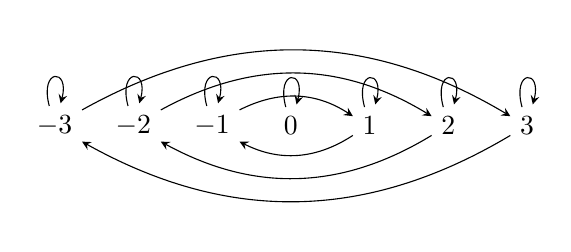
\begin{tikzpicture}[node distance=1.5cm,>=stealth,auto]
        \node (A-3) at (-3, 0) {$-3$};
        \node (A-2) at (-2, 0) {$-2$};
        \node (A-1) at (-1, 0) {$-1$};
        \node (A0) at (0, 0) {$0$};
        \node (A1) at (1, 0) {$1$};
        \node (A2) at (2, 0) {$2$};
        \node (A3) at (3, 0) {$3$};
        
        \draw[->] (A-3) edge[loop above] ();
        \draw[->] (A-2) edge[loop above] ();
        \draw[->] (A-1) edge[loop above] ();
        \draw[->] (A0) edge[loop above] ();
        \draw[->] (A1) edge[loop above] ();
        \draw[->] (A2) edge[loop above] ();
        \draw[->] (A3) edge[loop above] ();

        \draw[->] (A-3) to[bend left] (A3);
        \draw[->] (A3) to[bend left] (A-3);
        \draw[->] (A-2) to[bend left] (A2);
        \draw[->] (A2) to[bend left] (A-2);    
        \draw[->] (A-1) to[bend left] (A1);
        \draw[->] (A1) to[bend left] (A-1);
    \end{tikzpicture}
\newpage
	\section*{Tehtävä 2}
    Relaatio \(R\) edellisestä tehtävästä

    \begin{enumerate}
        \item[(a)] $R$ on refleksiivinen. Jokainen x \(\in\) \(A\) pätee \(x^2 = x^2\) pätee \(xRx\)
        \item[(b)] $R$ ei ole irrefleksiivinen. Koska x \(\in\) \(A\) pätee \(xRx\)
        \item[(c)] $R$ on symmetrinen. Jos \(xRy\), \(x^2 = y^2\) seuraa \(y^2 = x^2\) joten \(yRx\)
        \item[(d)] $R$ ei ole antisymmetrinen. Jos kaikilla \(x, y \in A\) pätee: jos  \(xRy\)  ja  \(yRx\) , niin  \(x = y\).
        Esimerkiksi  \(x = -1\)  ja  \(y = 1\), \(x^2 = x^2\) mutta \(x \neq y\) joten \(xRy\)  ja  \(yRx\) pätee
        \item[(e)] $R$ ei ole asymmetrinen. Koska \(R\) on symmetrinen.
        \item[(f)] transitiivinen?\newline
            Oletetaan:
            \begin{itemize}
                \item $xRy \implies x^2 = y^2$
                \item $yRz \implies y^2 = z^2$
            \end{itemize}
            Tavoite: \(xRz: x^2 = z^2\)
            \begin{itemize}
                \item $x^2 = y^2$
                \item $y^2 = z^2$
            \end{itemize}
            $\implies x^2 = y^2 = z^2$ \newline
            Joten $xRz$ pätee koska $x^2 = z^2$ eli $R$ on transitiivinen.
        \item[(g)] vertailullinen?\newline
        Relaatio  $R$  joukossa  $A$  on vertailullinen, jos kaikilla  $x, y \in A$  pätee joko  $xRy$  tai  $yRx$  tai molemmat.\newline
        Kokeillaan $x = -3$, madolliset  $y \in A :  -3, -2, -1, 0, 1, 2, 3$
        \begin{itemize}
            \item y = -2 : \( (-3)^2 = (-2)^2 \implies 9 \neq 4 \implies xRy \) ei päde
            \item yRx : \( (-2)^2 = (-3)^2 \implies 4 \neq 9 \implies yRx \) ei päde
        \end{itemize}
        $\implies$ on olemassa ainakin yksi pari  $(x, y) \in A \times A $, joille ei päde  $xRy$  eikä  $yRx$ joten $R$ ei ole vertailullinen.
        \item[(h)] $R$ on ekvivalenssirelaatio koska yllä on todettu että $R$ on refleksiivinen, symmetrinen ja transitiivinen.
    \end{enumerate}
    
    \newpage
	\section*{Tehtävä 3}
    Olkoot $R$ ja $S$ joukkojen $A$ ja $B$ välisiä relaatioita, toisin sanoen $R, S  \subset  A \times B$. Osoita, että
    \begin{enumerate}
        \item[(a)] $(R^{-1})^{-1} = R$ \newline
        $R^{-1} = \{ (b, a) \in B \times A \mid (a, b) \in R \}$\newline
        Käännetään relaatio $R^{-1}$:\newline
        $(R^{-1})^{-1} = \{ (a, b) \in A \times B \mid (b, a) \in R^{-1} \}$\newline
        Koska $(b, a) \in R^{-1}$ tarkoittaa $(a, b) \in R$\newline
        $\implies (R^{-1})^{-1} = \{ (a, b) \in A \times B \mid (a, b) \in R \}$\newline
        $\implies  (R^{-1})^{-1} = R$
        \item[(b)] $(R \cup S)^{-1} = R^{-1} \cup S^{-1} $
        \[
            \begin{aligned}
                (a,b) \in (R \cup S)^{-1} &\Longleftrightarrow (b,a) \in (R \cup S)\\
                &\Longleftrightarrow (b,a) \in R \text{ tai } (b,a) \in S\\
                &\Longleftrightarrow (a,b) \in R^{-1} \text{ tai } (a,b) \in S^{-1}\\
                &\Longleftrightarrow (a,b) \in R^{-1} \cup S^{-1}\\
            \end{aligned}
        \]
        \end{enumerate}


        \newpage
        \section*{Tehtävä 4}
        Määritellään kokonaislukujen joukossa $\mathbb{Z}$ relaatio $x \sim y \Longleftrightarrow x + y$ on parillinen luku. Osoita, että $\sim$ on ekvivalenssirelaatio.\newline
        Osoitetaan (tehtävä 2h mukaisesti):
        \begin{itemize}
            \item[\textbf{1)}] Refleksiivisyys: Jokaisella $x \in \mathbb{Z}$ pätee $x \sim x$
            \item[\textbf{2)}] Symmetrisyys: Jos $x \sim y$, niin $y \sim x$
            \item[\textbf{3)}] Transitiivisuus: Jos $x \sim y$ ja $y \sim z$, niin $x \sim z$ 
        \end{itemize}
    
        \begin{itemize}
            \item[\textbf{1)}]
            \[
                \begin{aligned}
                    x + x &= 2x\\
                    &\implies 2x \text{ on jaollinen kahdella joten $x + x$  on parillinen luku} \\
                    &\implies \text{Siis $x \sim x$ kaikilla } x \in \mathbb{Z} \\[5pt]
                \end{aligned}
            \]

            \item[\textbf{2)}]
            \begin{itemize}
                \item Oletetaan, että $x \sim y$, silloin $x + y$ on parillinen
                \item $x + y = 2k$ jollakin $k \in \mathbb{Z}$
                \item $y + x = x + y = 2k$
                \item Siis $y + x$ on parillinen, joten $y \sim x$
            \end{itemize}

            \item[\textbf{3)}]
            \begin{itemize}
                \item Oletetaan, että $x \sim y$ ja $y \sim z$, eli $x + y$ ja $y + z$ ovat parillisia lukuja
                \item Tällöin on olemassa kokonaisluvut $k, m \in \mathbb{Z}$ siten
                \begin{itemize}
                    \item $x + y = 2k$
                    \item $y + z = 2m$
                \end{itemize}
                \item Vähennetään toisistaan nämä yhtälöt:\newline
                    $(x + y) - (y + z) = 2k - 2m$ \newline
                    $x - z = 2(k - m)$
                \item Tästä seuraa $x - z$ on parillinen luku jolloin $x$ ja $z$ ovat joko parillisia tai parittomia jolloin myös $x + z$ on parillinen
                \item Näin ollen $x \sim z$
            \end{itemize}
        \end{itemize}
        Koska relaatio $\sim$ on refleksiivinen, symmetrinen ja transitiivinen, se on ekvivalenssirelaatio

\end{document}